\documentclass[tikz,border=6pt]{standalone}
\usepackage[T1]{fontenc}
\usepackage{lmodern}
\usepackage{amsmath,amssymb}
\usetikzlibrary{arrows.meta,calc,positioning,shapes.geometric,patterns,decorations.pathmorphing,backgrounds,fit}
\definecolor{ink}{HTML}{173948}
\definecolor{flow}{HTML}{167D9A}
\definecolor{heat}{HTML}{B75A23}
\definecolor{measure}{HTML}{70518A}
\definecolor{pale}{HTML}{EAF2F5}
\definecolor{muted}{HTML}{526571}
\definecolor{green}{HTML}{2E8665}
\tikzset{every node/.style={font=\sffamily\small,text=ink},
 equipment/.style={draw=ink,line width=1pt,fill=pale,rounded corners=2pt},
 process/.style={draw=flow,line width=1.1pt,-{Latex[length=2.4mm]}},
 signal/.style={draw=measure,dashed,line width=.9pt,-{Latex[length=2mm]}},
 thermal/.style={draw=heat,line width=1.1pt,-{Latex[length=2.3mm]}},
 labelbox/.style={fill=white,inner sep=2pt,font=\sffamily\footnotesize,align=center},
 annotation/.style={font=\sffamily\footnotesize,text=muted,align=left},
 panel/.style={draw=ink!20,fill=ink!2,rounded corners=3pt,inner sep=7pt,align=left},
 sensor/.style={circle,draw=measure,fill=white,line width=.8pt,minimum size=8mm,inner sep=1pt,font=\sffamily\scriptsize,align=center},
 box/.style={equipment,minimum width=3cm,minimum height=1.2cm,align=center}}
\newcommand{\atlasheader}[2]{\node[anchor=north west,font=\sffamily\bfseries\LARGE]at(0,0){#1};\node[anchor=north west,font=\sffamily\small,text=muted]at(0,-.75){#2};\draw[ink!25](0,-1.25)--(26,-1.25);}
\newcommand{\atlasfooter}[1]{\draw[ink!25](0,-15.8)--(26,-15.8);\node[anchor=north west,annotation,text width=25.8cm]at(0,-16){#1\\Original explanatory drawing for ThermoFuzzy-PID. Source traceability: Cordeiro (UFC, 2021), documented repository equations and explicit reconstruction choices.};}

\newcommand{\rulegrid}[3]{%
\begin{scope}[shift={(#1,-6.4)}]
\node[anchor=south west,font=\sffamily\bfseries]at(0,.85){#2};
\foreach \j/\term in {0/NB,1/NM,2/NS,3/Z,4/PS,5/PM,6/PB}{\node[font=\sffamily\footnotesize]at(\j+.5,.35){\term};\node[font=\sffamily\footnotesize,anchor=east]at(-.12,-\j*.59-.295){\term};}
\foreach \j in {1,5}{\fill[ink!10](\j,0)rectangle(\j+1,-4.13);}
\foreach \j in {0,...,7}{\draw[ink!35](\j,0)--(\j,-4.13);}
\foreach \j in {0,...,7}{\draw[ink!35](0,-\j*.59)--(7,-\j*.59);}
\foreach \v[count=\n from 0]in{#3}{\pgfmathtruncatemacro{\col}{mod(\n,7)}\pgfmathtruncatemacro{\row}{\n/7}\node[font=\sffamily\footnotesize]at(\col+.5,-\row*.59-.295){\v};}
\node[annotation,anchor=north]at(3.5,-4.35){Columns: $|e|$ category; rows: signed $\Delta e$ category};
\end{scope}}
\begin{document}
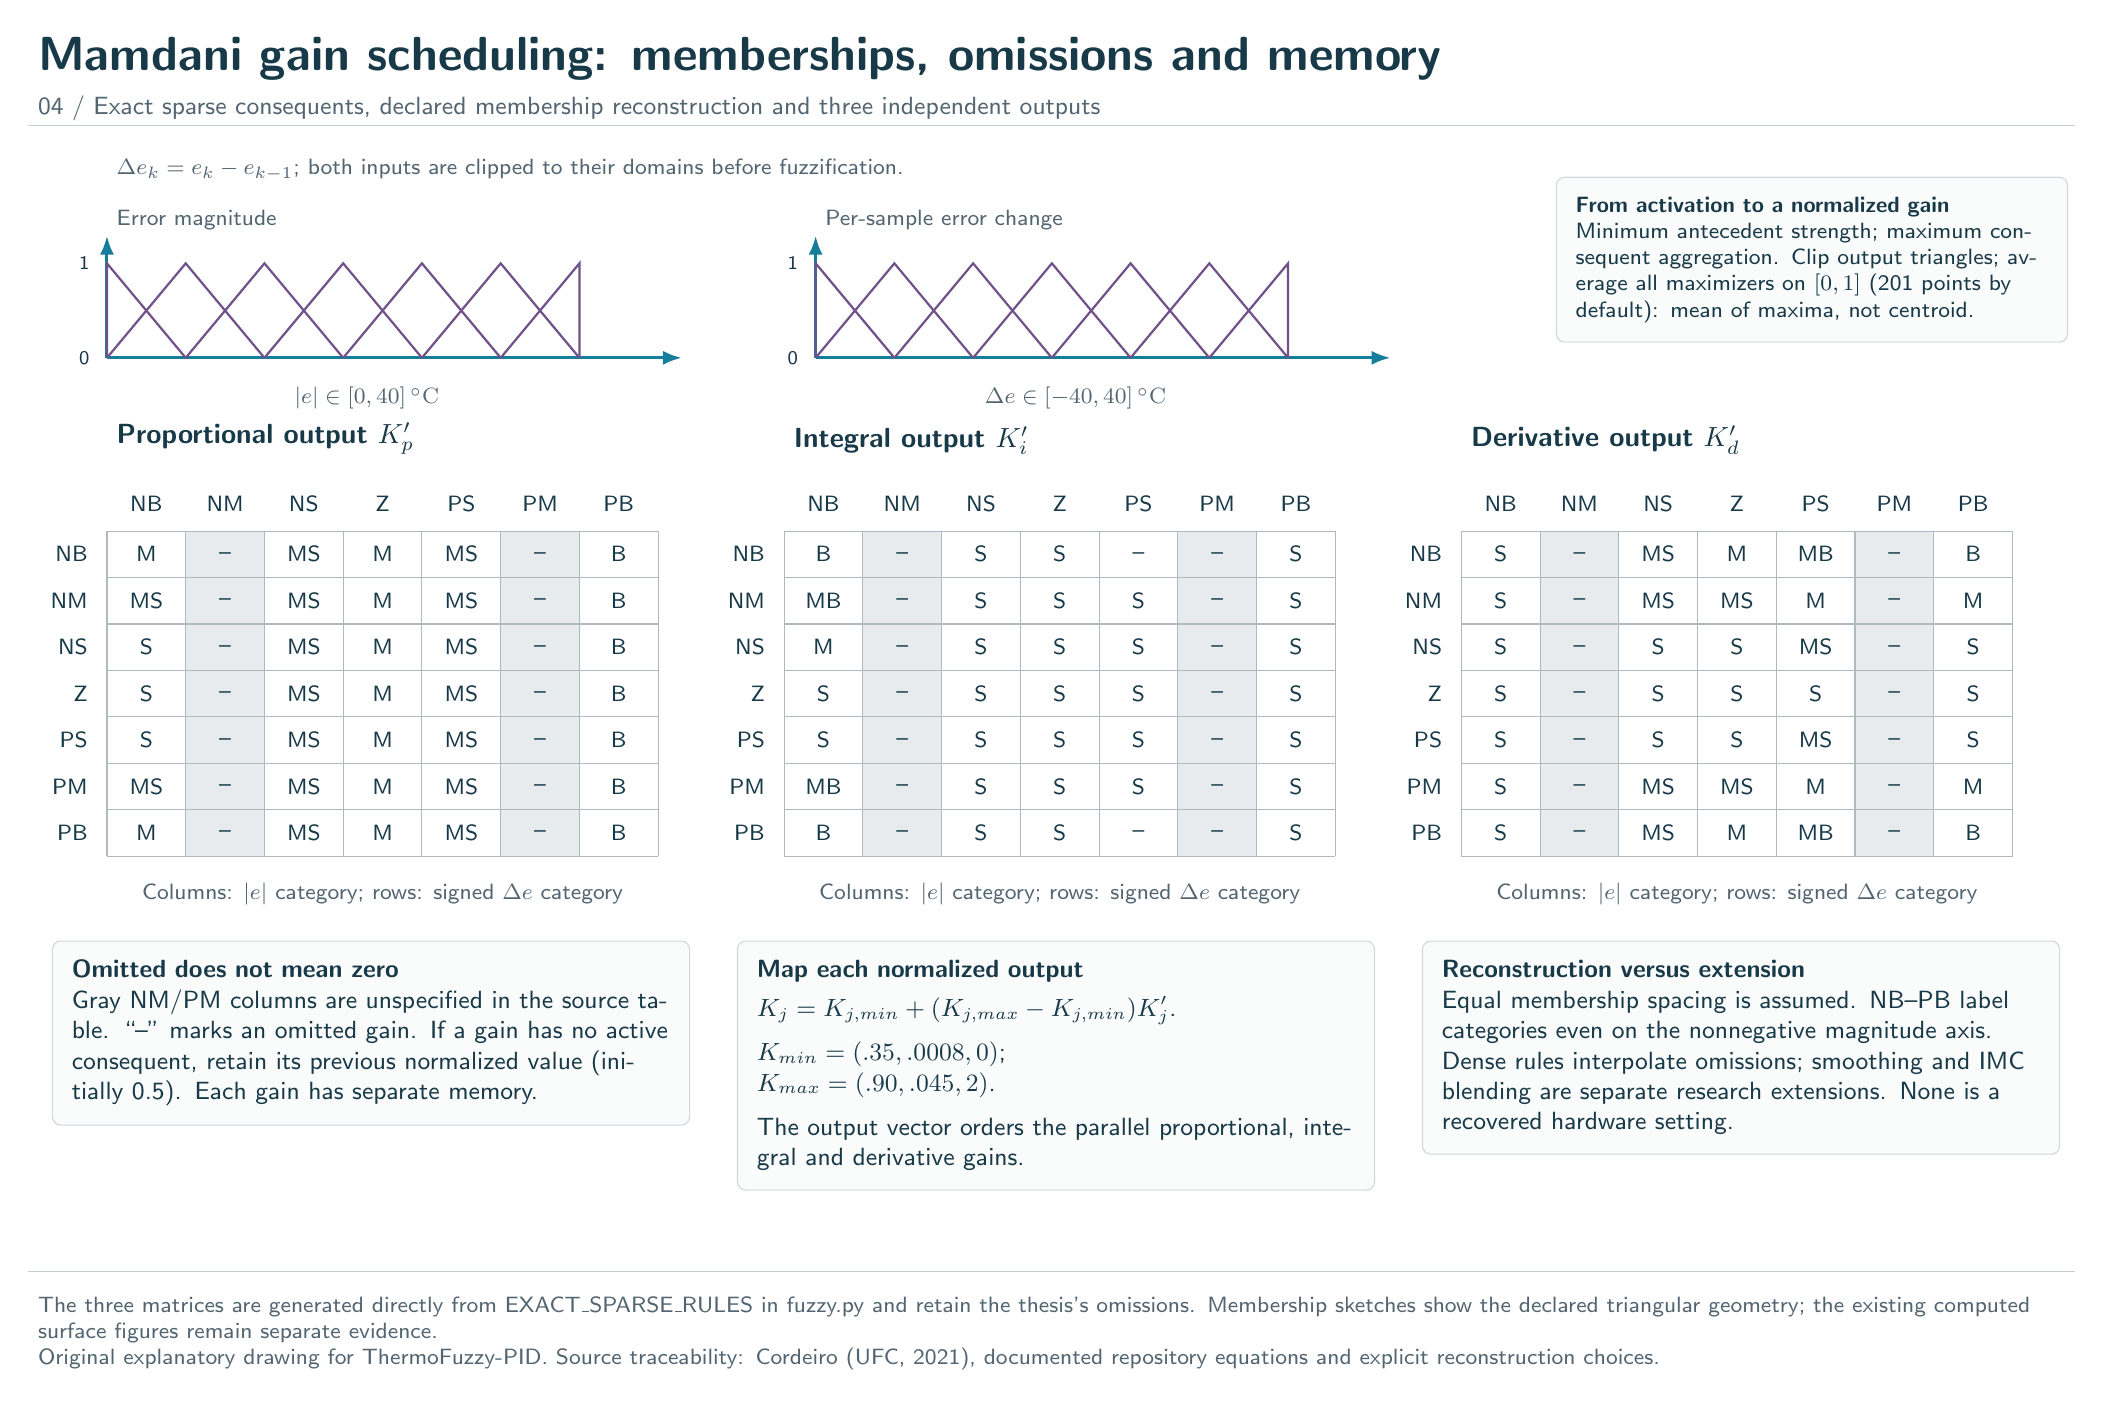
\begin{tikzpicture}[x=1cm,y=1cm]
\atlasheader{Mamdani gain scheduling: memberships, omissions and memory}{04 / Exact sparse consequents, declared membership reconstruction and three independent outputs}
\foreach \origin/\caption/\domain in {1.0/Error magnitude/{$|e|\in[0,40]\,^{\circ}\mathrm C$},10.0/Per-sample error change/{$\Delta e\in[-40,40]\,^{\circ}\mathrm C$}}{
 \begin{scope}[shift={(\origin,-4.2)}]
 \draw[process](0,0)--(7.3,0);\draw[process](0,0)--(0,1.55);
 \foreach \j in {0,...,6}{\draw[measure,line width=.8pt]({max(0,\j-1)},0)--(\j,1.2)--({min(6,\j+1)},0);}
 \node[annotation,anchor=south west]at(0,1.5){\caption};
 \node[annotation,anchor=north]at(3.3,-.25){\domain};
 \node[font=\sffamily\scriptsize,anchor=east]at(-.1,1.2){1};
 \node[font=\sffamily\scriptsize,anchor=east]at(-.1,0){0};
 \end{scope}}
\node[panel,anchor=north west,text width=6.0cm,font=\sffamily\footnotesize]at(19.4,-1.9){\textbf{From activation to a normalized gain}\\Minimum antecedent strength; maximum consequent aggregation. Clip output triangles; average all maximizers on $[0,1]$ (201 points by default): mean of maxima, not centroid.};
\node[annotation,anchor=north west]at(1,-1.55){$\Delta e_k=e_k-e_{k-1}$; both inputs are clipped to their domains before fuzzification.};
% Generated from EXACT_SPARSE_RULES; do not edit this table manually.
\rulegrid{1.0}{Proportional output $K_p^{\prime}$}{M,--,MS,M,MS,--,B,MS,--,MS,M,MS,--,B,S,--,MS,M,MS,--,B,S,--,MS,M,MS,--,B,S,--,MS,M,MS,--,B,MS,--,MS,M,MS,--,B,M,--,MS,M,MS,--,B}
\rulegrid{9.6}{Integral output $K_i^{\prime}$}{B,--,S,S,--,--,S,MB,--,S,S,S,--,S,M,--,S,S,S,--,S,S,--,S,S,S,--,S,S,--,S,S,S,--,S,MB,--,S,S,S,--,S,B,--,S,S,--,--,S}
\rulegrid{18.2}{Derivative output $K_d^{\prime}$}{S,--,MS,M,MB,--,B,S,--,MS,MS,M,--,M,S,--,S,S,MS,--,S,S,--,S,S,S,--,S,S,--,S,S,MS,--,S,S,--,MS,MS,M,--,M,S,--,MS,M,MB,--,B}

\node[panel,anchor=north west,text width=7.6cm]at(.3,-11.6){\textbf{Omitted does not mean zero}\\Gray NM/PM columns are unspecified in the source table. ``--'' marks an omitted gain. If a gain has no active consequent, retain its previous normalized value (initially 0.5). Each gain has separate memory.};
\node[panel,anchor=north west,text width=7.6cm]at(9.0,-11.6){\textbf{Map each normalized output}\\[3pt]
$K_j=K_{j,min}+(K_{j,max}-K_{j,min})K'_j$.\\[5pt]
$K_{min}=(.35,.0008,0)$;\\$K_{max}=(.90,.045,2)$.\\[5pt]
The output vector orders the parallel proportional, integral and derivative gains.};
\node[panel,anchor=north west,text width=7.6cm]at(17.7,-11.6){\textbf{Reconstruction versus extension}\\Equal membership spacing is assumed. NB--PB label categories even on the nonnegative magnitude axis. Dense rules interpolate omissions; smoothing and IMC blending are separate research extensions. None is a recovered hardware setting.};
\atlasfooter{The three matrices are generated directly from EXACT\_SPARSE\_RULES in fuzzy.py and retain the thesis's omissions. Membership sketches show the declared triangular geometry; the existing computed surface figures remain separate evidence.}
\end{tikzpicture}
\end{document}
